\documentclass[a4paper]{IEEEtran}

\usepackage{xcolor}
\usepackage{hyperref}
\usepackage[utf8]{inputenc}
\usepackage[pdftex]{graphicx} 

\newcommand\TODO[1]{\textcolor{red}{TODO:#1}}
\newcommand\todo[1]{\TODO{#1}}
\newcommand\cn{\textcolor{red}{[citation needed]}}

\title{Indiana Jones and the Quest for the Extraterrestrial Liaison!}

\author{
    Rune Holmgren,
    Torbjørn Langland
}

\begin{document}

\maketitle

\begin{abstract}
    \todo{ Compulsory (means that it is specified in the Term Project in description of report set up, and at this very location). Create a fitting abstract here. Also create a FRONT PAGE. Yes, you didn't read wrong. I wrote in capital letters. If we miss this now, we must indeed be quite stupid...}
\end{abstract}

\section{Front Page}
\todo{ Compulsory. Again, create FRONT PAGE. Didn't immediatly know better how to put this in, so just added this as first section (NOOB!). }

\section{Introduction}
\todo{ Compulsory. Introduction that explains what to expect of the report. Introduction of the term project should be covered in abstract? }

\section{Table of Contents}
\todo{ Compulsory. Must generate. I leave that to you, Rune}

\section{Problem to be solved. Method.}
\todo{ Insert chapter introduction here. }
\break
\break
\todo{ Describe the student satelite }
\break
\break
\todo{ Describe the communication syste. Describe the need for voters }
\break
\break
\todo{ Describe the idea for the Liaison system. Treat it like a black box and explain what it is supposed to do.}
\break
\break
\todo{ Include figure(s) from pages 4-5 in order to explain the wanted functionality. }
\break
\break
\todo{ Also mention that the solution to this problem is split into different sub-sproblems? }

\section{ Solution to the problem}
\todo{ Term project specifies that the answer to all subproblems is to be explained. We should therefore split these into subsection. }
\break
\break
\todo{ Insert chapter introduction here. Remember to mention that we used Active HDL and Synplify Pro.}
\break
\break
\todo{ WARNING: Points of Term project report specifiaction sort of overlaps. Perhaps own chapters for testing and verification, or only the sub-chapters of this one are enough. Discuss, choose, live, rule, win!} 

\subsection{Sub-Problem 1: State analysis}
\todo{ Insert the State Machine figure here. Explain it, and choices the group has done in the design. }

\subsection{Sub-Problem 2: One-Bit voter}
\todo{ Explain the implementation of the One-bit Voter.}
\break 
\break
\todo{ Explain test results. Include figures. OR explain in section "Testing and verification" }
\break
\break
\todo{ Explain synthesis results: Estimated Frequency and generated LUTs}
\break
\break
\todo{ Find out if one or both voters must be explained (at least mention synthesis results of the second one). }

\subsection{Sub-Problem 3: 8-Bit voter}
\todo{ Explain the different options for implementations. Include figures. (Can screenshot from technical note. Yehaa, there was some use from that long night after all :P ) }
\break
\break
\todo{ Explain the chosen architecture. Include figure (screenshot it from the presentation). }
\break
\break
\todo{ Explain test results. Include figures. OR explain in section "Testing and verification" }
\break
\break
\todo{ Explain synthesis results}
\break
\break


TEXT
\begin{figure}[h!]
  \centering
      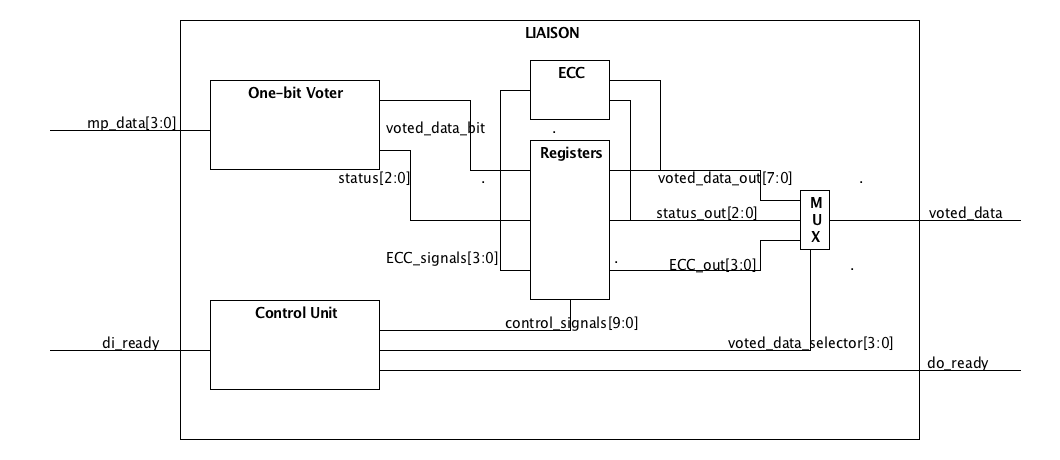
\includegraphics[width=0.5\textwidth]{Figures/ArchitectureFinal}
  \caption{Chosen architecture for the 8-bit Voter}
  \label{fig:ArchitectureFinal}
\end{figure}
TEXT
\begin{figure}[h!]
  \centering
      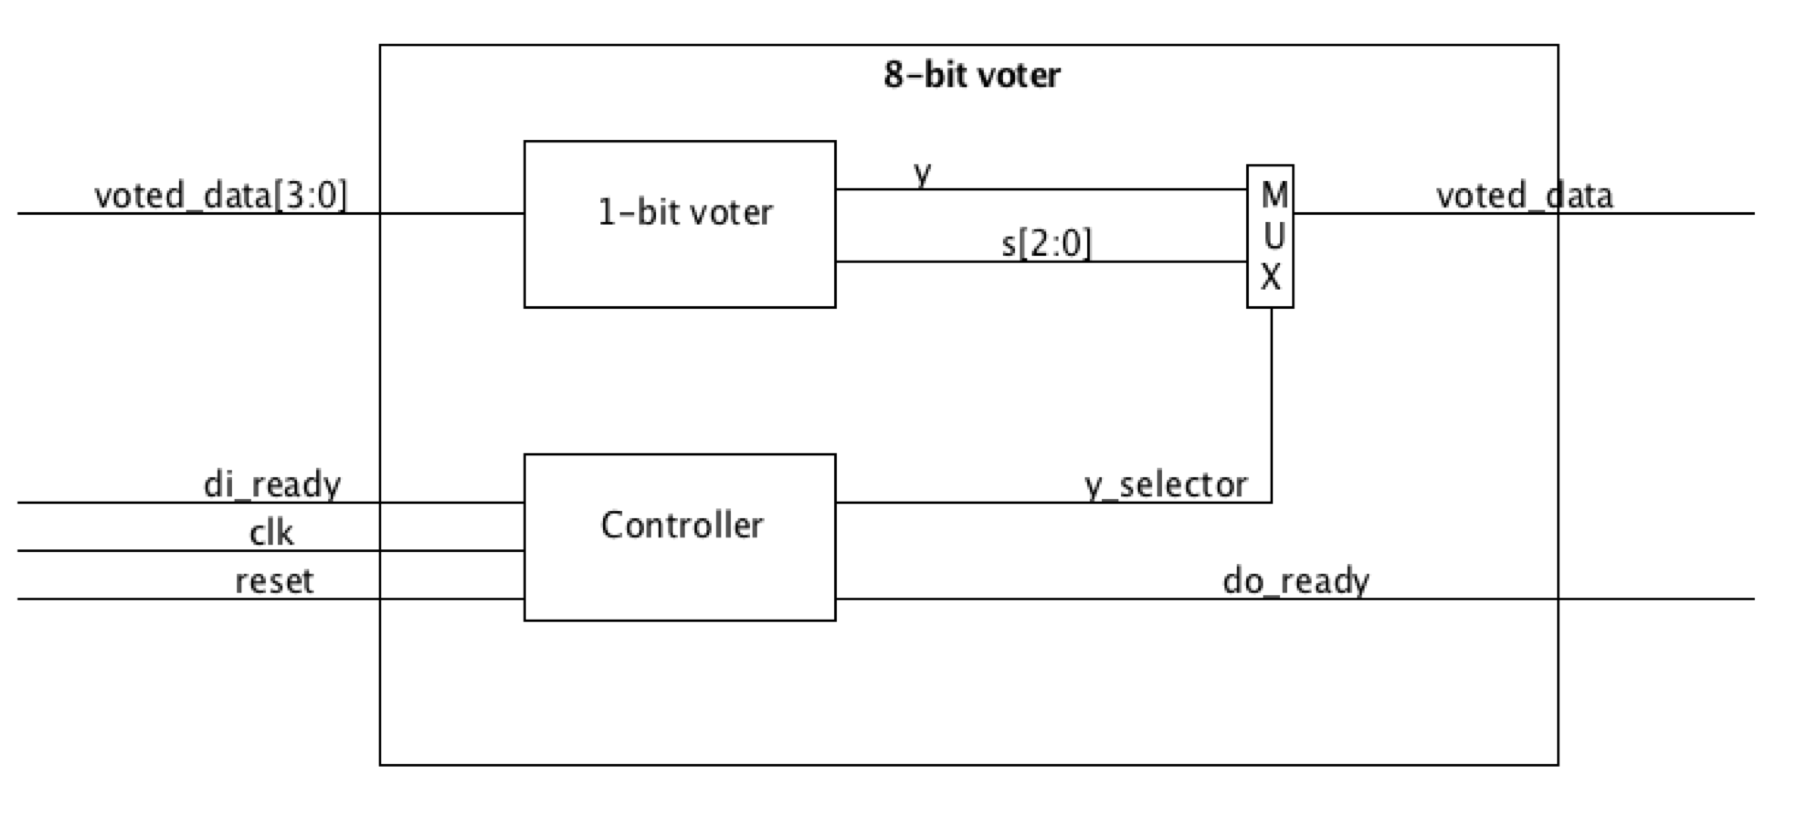
\includegraphics[width=0.5\textwidth]{Figures/ArchitectureOption2}
  \caption{Chosen architecture for the 8-bit Voter}
  \label{fig:ArchitectureOption2}
\end{figure}
TEXT
\begin{figure}[h!]
  \centering
      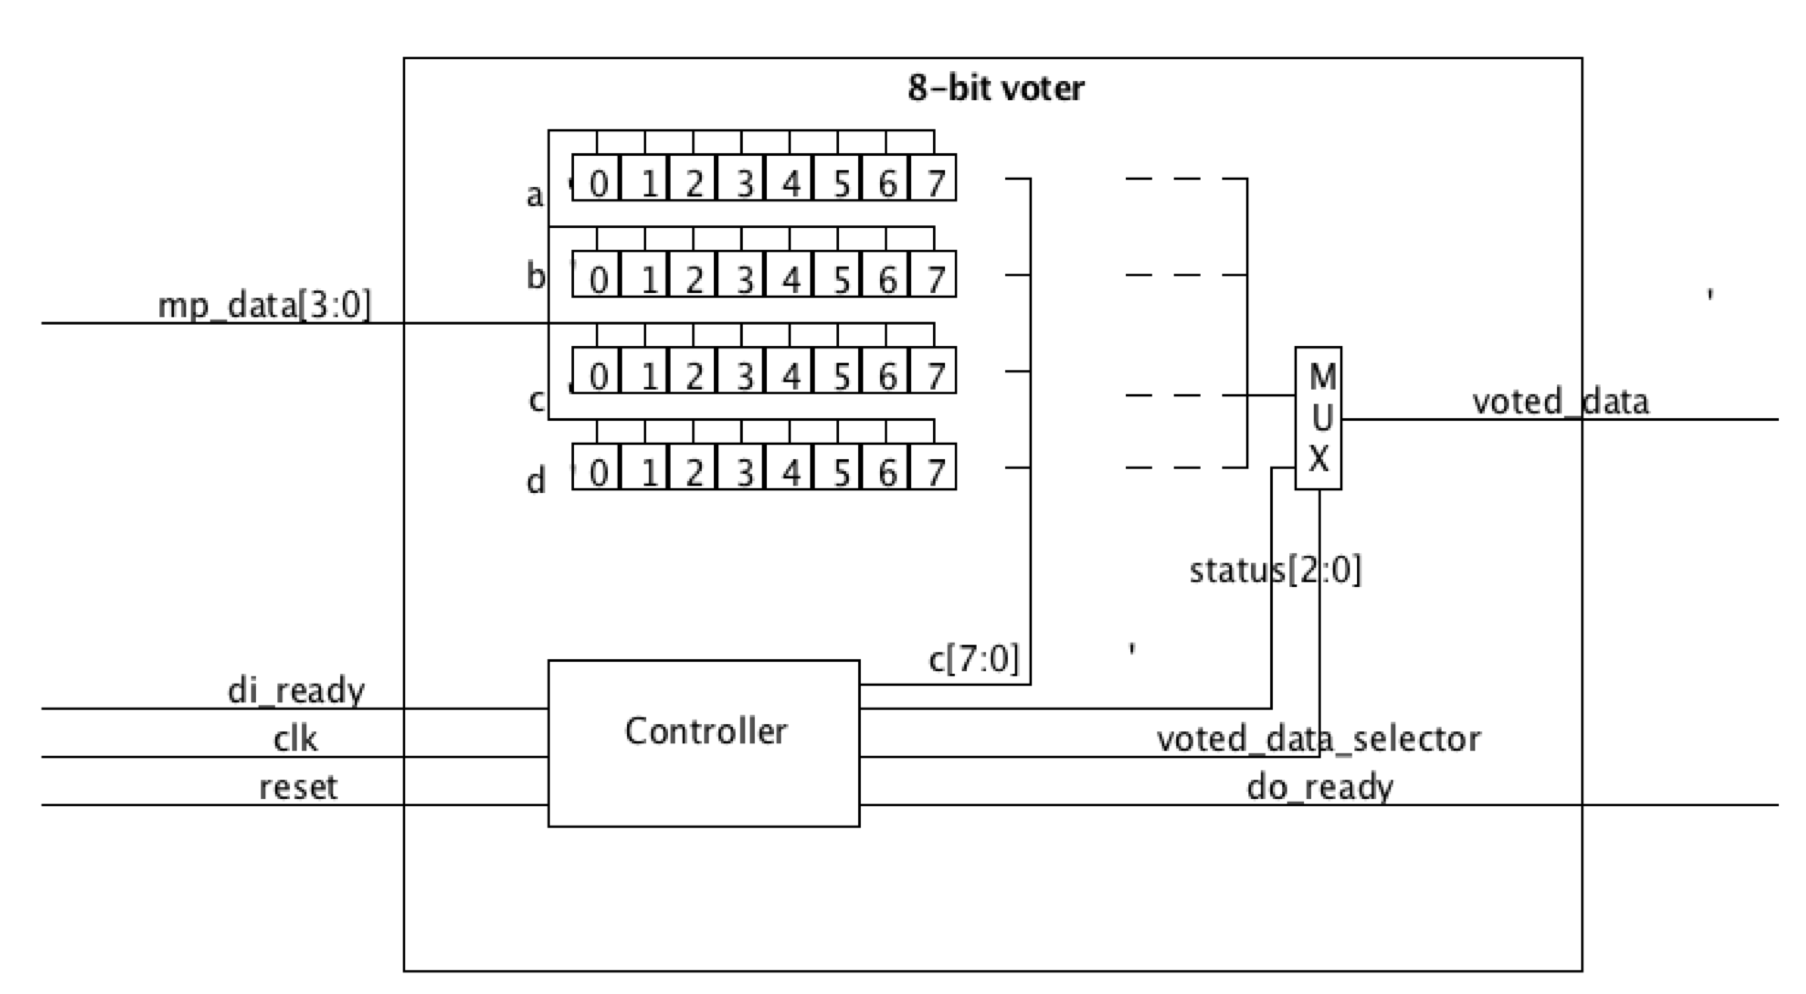
\includegraphics[width=0.5\textwidth]{Figures/ArchitectureOption3}
  \caption{Chosen architecture for the 8-bit Voter}
  \label{fig:ArchitectureOption3}
\end{figure}

TEXT
\subsubsection{ Details of the 8-bit voter}.
\todo{ Detail the controller.}
\break
\break
\todo{ Detail the Registers.}
\break
\break
TEXT
\begin{figure}[h!]
  \centering
      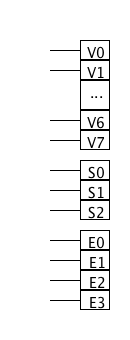
\includegraphics[width=0.5\textwidth]{Figures/Registers}
  \caption{Chosen architecture for the 8-bit Voter}
  \label{fig:Registers}
\end{figure}

\subsection{Sub-Problem 4: Error Correction Circuit}
\todo{ Explain how the ECC is implemented, perhaps explain Hamming Coding. Include figure (screenshot it from the presentation). }
\break
\break
\todo{ The term project states: "Your final report should comment on the use of intellectual property-modules and the reasoning behind why this scheme is appropriate." To this.}
\break
\break
\todo{ Explain test results. Include figures. OR explain in section "Testing and verification" }
\break
\break
\todo{ Explain synthesis results}

\subsection{Sub-Problem 5: Analysis of error probabilities}
\todo{ Explain briefly the theory behind a microcontroller failure. }
\break
\break
\todo{ Explain the mathematical expressions for P(Max(1)), P(Max(2)), P(Least(3), and the results from calculating MTTF.}
\break
\break
\todo{ Refer to Appendix C for full calculation.}

\section{ Testing and verification }
\todo{ Either explein the testing and verification here, or do it seperately in the subchapters of the previous chapter. Delete this chapter if we choose the other solution. I vote this one. But if we do so, for consistensy we may then have to create a independent chapter for Synthesis }
\break
\break
\todo{ Insert introduction }

\subsection{ Tests and verification of One-Bit Voter}
\todo{ Explain choice of test bench. Explain why it gives full coverage}
\break
\break
\todo{ Explain test results. Include screenshot (Uh... the provided test bench is not of that kind).}

\subsection{ Control Unit}
\todo{ Explain choice of test bench. Explain why it gives full coverage}
\break
\break
\todo{ Explain test results. Include screenshot. }

\subsection{ ECC }
\todo{ Explain choice of test bench. Explain why only partial coverage is enough. }
\break
\break
\todo{ Explain test results. Include screenshot. }

\subsection{ Liasion }
\todo{ Explain choice of test bench. Explain why only partial coverage is enough. }
\break
\break
\todo{ Explain test results. Include figure. (Screenshot it from the presentation) }

\section{Synthesis }
\todo{ Decide whether we should have a own chapter for this or not. If we choose this option for testing and verification, we should do this for synthesis as well in the name of consistency. }
\break
\break
\todo{ Insert introduction }
\break
\break
\todo{ Refer to Appendix B for schematics. Both RTL and that other one. }


\section{Conclusion}
\todo{ Compulsory. Have a good wrap up, somehow. }

\section{Acknowledgements (optional)}

Indiana Jones. Should also mention group 2 and the student assistant.

\section{ Other problems/needs to be solved:}
\subsection{ Appendixes}
\todo{ Appendix A: Project codes }
\break
\break
\todo{ Appendix B: Synthesis Schematics. Both RTL and that other type, propose top architecture first then One-bit-Voter, Controller, Registers and ECC. RTL first then that other type.}
\break
\break
\todo{ Appendix C: The Probability Calculation. I got it covered. }
\subsection{ Other problems/needs:}
\todo{ Find out where to list up time spent in the project.}

\bibliographystyle{plain}
\nocite{*}

\end{document}
